%!TEX TS-program = pdflatex
%!TEX root = tesi.tex
%!TEX encoding = UTF-8 Unicode

%\begin{figure}[ht] % TODO remove me
%  \begin{center}
%    \begin{tabular}{ccc}
%
%  \begin{subfigure}{.3\linewidth}
%    \centering\includegraphics[width=\textwidth]{example-image}
%    \caption{}
%  \end{subfigure} &
%
%    \end{tabular}
%    \caption{Alcune carcasse Conformi}
%    \label{fig:esempi_conformi}
%  \end{center}
%\end{figure}



\chapter{Gli Autoencoder}

Breve intuizione sugli AE
\todo[inline]{TODO recap capitolo}
\todo[inline]{TODO recap capitolo}
\todo[inline]{TODO recap capitolo}
\todo[inline]{TODO recap capitolo}
\todo[inline]{ipotizzo almeno 5 righe}

\section{La Struttura di un Autoencoder}
Un \textit{Autoencoder}(AE) è un particolare tipo di rete neurale.
Può essere diviso in due componenti: il primo viene chiamato \textit{encoder}, mentre il secondo prende il nome di \textit{decoder}.
Lo scopo dell'\textit{encoder} è codificare il dato in ingresso in una versione compressa.
Sia $n$ la dimensionalità dell'\textit{input}.
Quando il dato raggiunge il collo di bottiglia dell'AE, ovvero la parte centrale della rete, ha raggiunto il livello di massima compressione, sia $m$ la sua nuova dimensionalità con $m<n$.
Lo spazio $m$-dimensionale in cui l'informazione è stata mappata viene chiamato spazio latente o spazio nascosto.
Ora il dato può essere decompresso dal \textit{decoder}, in questo modo verrà riportato alle sue dimensioni originali, cioè mappato nello spazio $n$-dimensionale di partenza.

Visto dall'esterno, il compito di un \textit{autoencoder} è quello di ritornare un valore il più simile al dato in ingresso.
Durante l'allenamento, fissato $m$ con un valore che dipende dalla forma della rete, si vuole trovare il miglior spazio latente possibile.
Dove con migliore si intende quello spazio di cardinalità $m$ che permette di mantenere tutte le informazioni caratterizzanti dell'input.
Riformulando quanto detto: un'\textit{autoencoder} può essere visto come una funzione $f$ rassomigliante la funzione identità, ma al cui intero c'è un vincolo tale da rendere il compito di restituzione dell'\textit{input} non banale.

Come viene spiegato da Andrew Ng in \cite{ng_sparse_ae}, gli \textit{autoencoder} fanno parte degli algoritmi di apprendimento non supervisionato.
Cioè di quella classe di algoritmi, in contrapposizione a quelli ad apprendimento supervisionato, che non ha bisogno di dati etichettati; anzi vengono usati proprio per trovare nuovi pattern e correlazioni tra gli elementi del \textit{dataset}.
Come gli algoritmi \textit{K-Means} e \textit{DBSCAN}, entrambi di \textit{clustering}, permettono di raggruppare nuvole di punti con caratteristiche simili. % TODO citare?
%I gruppi così creati possono far risaltare degli andamenti dei dati 
Un AE è non supervisionato perché, a priori, non conosciamo la forma che verrà data allo spazio latente. % TODO espandere?

Gli \textit{autoencoder} più semplici sono composti da due strati densamente connessi di neuroni: il primo funge da \textit{encoder} ed ha un numero di unità pari alla dimensione dello spazio latente; il secondo ha tante unità quanto la dimensione dell'\textit{input}, quindi funge da \textit{decoder}.
L'architettura appena descritta può essere osservata in figura~\ref{fig:semplice_ae}, notare la tipica forma a clessidra.

\begin{figure}[ht] % TODO rifare con tikz
  \begin{center}
    %\centering\includegraphics[width=.4\textwidth]{example-image}
    \centering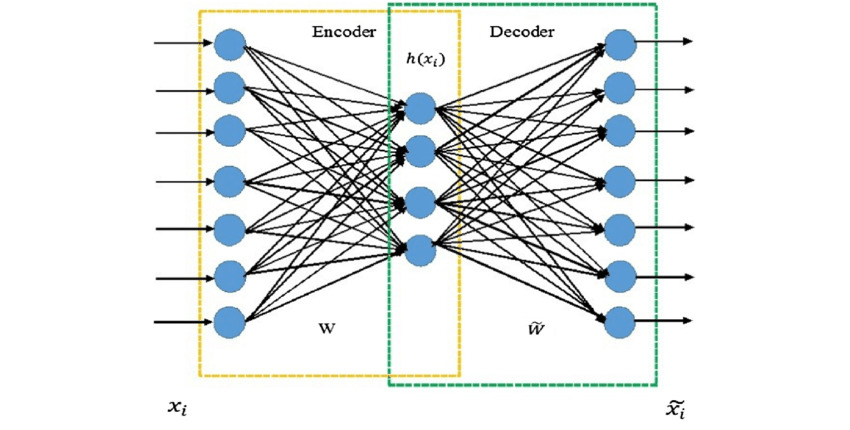
\includegraphics[width=\textwidth]{simple_ae}
  \end{center}
  \caption{Architettura di un semplice \textit{autoencoder}}
  \label{fig:semplice_ae}
\end{figure}


Facendo sempre rifermento a \cite{ng_sparse_ae}, un neurone è un'unità computazionale che prende in \textit{input} un vettore $x$ di elementi $x_i$ con $i=1,2,3,\dots,n$ e che ritorna $h_{W,b}(x) = f(W^Tx) = f(\sum_{i=1}^{n} W_i x_i + b)$.
Dove $h_{W,b}(x)$ è un generatore di ipotesi non-lineare, con parametri $W$ e $b$ che possono adattarsi al \textit{dataset}.
I pesi del neurone vengono salvati in $W$, vettore con tanti elementi quanti quelli di $x$.
%bias = pregiudizio
Il valore $b$ viene detto \textit{bias} è una quantità che verrà sempre sommata al risultato del prodotto riga per colonna tra $W$ e $x$.
% TODO fare figura a cui posso riferirmi per spiegare dove sono messi i pesi
La funzione $f$ è chiamata funzione di attivazione.
La funzione sigmoidea viene utilizzata spesso come funzione di attivazione, è definita come:
\begin{equation*}
  f(z) = \frac{1}{1 + exp(-z)}
\end{equation*} %TODO fare plot?
Notare come $f(z)$ sia una una funzione da $\mathbb{R}$ in $[0,1]$.
Ciò risulta utile soprattutto se il compito del neurone è dividere gli \textit{input} in due classi distinte, cioè $0$ e $1$, basterà verificare se $f(z)>0.5$.
In caso affermativo l'\textit{input} verrà associato alla classe con etichetta $1$, altrimenti a $0$.
Un'altra funzione di attivazione, molto utilizzata nei nodi interni delle reti, viene chiamata \textit{ReLU} ed è definita come:
\begin{equation*}
  f(z) = max(0,z)
\end{equation*} %TODO fare plot?
La funzione \textit{ReLU}, che significa \textit{Rectified Linear Unit}, è stata pensata per simulare ciò che avviene in un vero neurone:
fino a che il segnale in ingresso non supera una certa soglia il neurone rimane inattivo, ciò corrisponde a valori di $z$ inferiori o pari a zero;
appena il segnale diventa abbastanza intenso, allora il neurone inizia a trasmettere.
All'aumentare della potenza del segnale in ingresso corrisponde un aumento proporzionale anche in uscita.

Quando uno strato della rete è composto da più neuroni, ciascuno di essi riceverà una copia di $x$ e ritornerà un \textit{output} in base ai propri $W$ e $b$.
%In figura~\ref{fig:semplice_ae} si può notare come gli $x_i$ vengano distribuiti su tutti i nodi del primo strato e come il loro risultato venga a sua volta distribuito sulle altre unità.
Dato che il numero di connessioni cresce rapidamente, essendo pari a $n*m$ per ogni strato (con $n$ la dimensione del vettore in ingresso ed $m$ di quello in uscita), questi strati vengono chiamati densamente connessi o, più semplicemente, densi.

Dato che l'\textit{input} di una funzione d'attivazione è il risultato del prodotto vettoriale tra $x$ e i pesi del neurone, bisogna chiarire come questi pesi vengano aggiustati.
In altre parole bisogna definire in che modo la rete venga allenata.

Facendo rifermento a quanto spigato in \cite{ng_deep_learning}, si consideri una rete il cui scopo è determinare se in un'immagine è raffigurato un gatto.
Il caso affermativo corrisponde a 1, quello negativo a 0.
Se si effettua una linearizzazione dell'immagine in un vettore $x$, è possibile fornire il vettore appena creato in ingesso alla rete neurale in figura~\ref{fig:nn}.
\begin{figure}[ht]
  \begin{center}
    \centering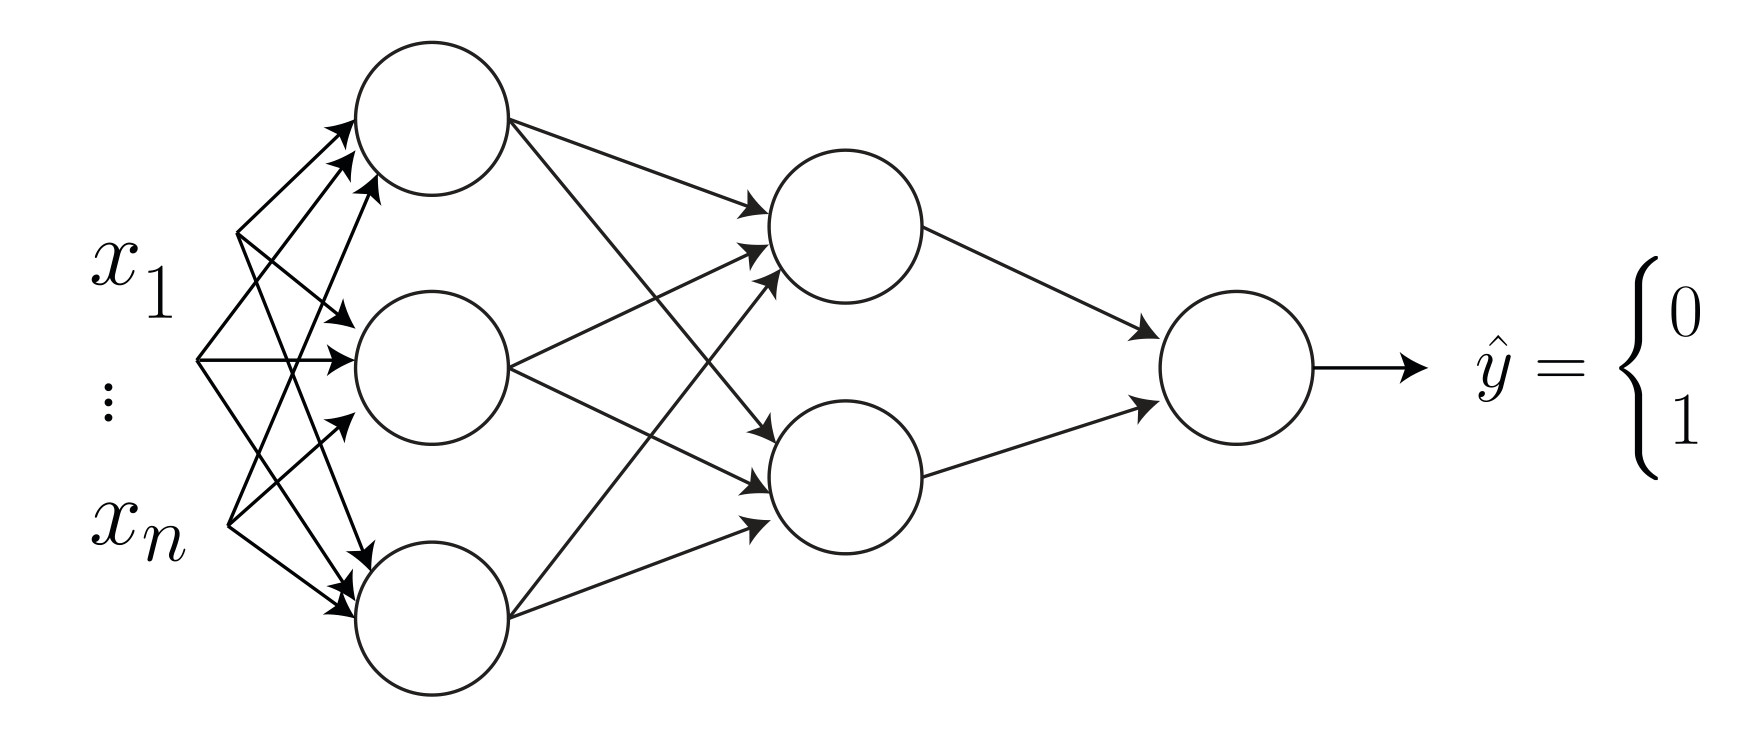
\includegraphics[width=0.55\textwidth]{nn}
  \end{center}
  \caption{Semplice rete neurale}
  \label{fig:nn}
\end{figure}
Il \textit{dataset} sarà quindi formato da vettori $x$ etichettati con valori $y \in {0,1}$.
Si fa notare che l'allenamento di una rete neurale può essere ricondotto ad un problema di minimizzazione, in cui si vuole minimizzare le predizioni sbagliate.
L'algoritmo con cui si allenano le reti neurali viene chiamato \textit{backpropagation} e può essere diviso in due momenti:
nel primo i calcoli vengono effettuati da sinistra a destra, così da ottenere la predizione $\hat y$;
nel secondo, dopo aver calcolato l'errore della predizione, i pesi, partendo da destra, vengono aggiornati.
In questo esempio lo scarto verrà calcolato usando la funzione di costo logaritmica, definita come:
\begin{equation} \label{eq:log-cost}
  L(\hat y, y) = - ln(\hat y) - (1-y) ln(1- \hat y)
\end{equation}
Si può notare come l'equazione~\ref{eq:log-cost} tenda a 0 quando i valori di $\hat y$ e $y$ sono simili, mentre tenderà a valori molto grandi se la predizione non è corretta; infatti $L(\hat y, y)= + \infty$.
A questo punto i pesi di ogni \textit{layer} $l$ possono essere aggiornati con:
\begin{align} \label{eq:grad-desc}
  W^{[l]} &= W^{[l]} - \alpha \frac{\partial L}{\partial W^{[l]}} \\ \\
  b^{[l]} &= b^{[l]} - \alpha \frac{\partial L}{\partial b^{[l]}}
\end{align}
Il parametro $\alpha$ prende il nome di tasso di apprendimento, in inglese \textit{learning rate}, mentre $\partial L / \partial W^{[l]} $ e $\partial L / \partial b^{[l]}$ sono dei gradienti.
In pratica si sta applicando l'algoritmo di \textit{gradient descent} ad ogni neurone della rete.
L'intuizione con cui quest'ultimo opera è sfruttare la derivata di una funzione $f(x)$ per avvicinarsi, al crescere delle iterazioni, al suo minimo.
Se il segno della derivata $f'(x)$ è negativo significa che il valore di $f$, calcolato nell'immediato intorno destro di $x$, sarà minore di $f(x)$.
Viceversa, se la derivata ha segno positivo, $f$ sarà più piccola per valori a sinistra di $x$.

Nell'equazione~\ref{eq:grad-desc} si può vedere come il valore del gradiente vada a modificare i pesi, proprio con le modalità appena descritte.
Ora anche lo scopo del parametro $\alpha$ risulta più chiaro: definisce quanto aggiornare i pesi del neurone.
Trovare un adeguato tasso di apprendimento è fondamentale se si vuole alleare correttamente una rete.
Si vede chiaramente come valori troppo piccoli di $\alpha$ fanno in modo che i pesi non vengono aggiornati affatto, mentre valori troppo grandi potrebbero portare l'algoritmo di \textit{backpropagation} a non convergere. % TODO va giustificato?

Chiarito il modo in cui la rete apprende, resta da specificare il modo in cui il \textit{dataset} venga fornito alla rete durante l'allenamento.
Un allenamento è composto da svariate epoche ed ogni epoca è suddivisa in \textit{batch}.
Un \textit{batch} è un gruppo di elementi, questi gruppi sono creati in modo da formare una partizione del \textit{dataset}.
Dopo che la rete ha elaborato i dati contenuti in un singolo \textit{batch} viene utilizzato l'algoritmo di \textit{backpropagation} per aggiornane i pesi.
Un epoca si conclude soltanto quando questo procedimento è stato effettuato per tutti i gruppi.
Quindi ad ogni epoca corrisponde la predizione e l'aggiornamento dei pesi per ciascun elemento del \textit{dataset}.
Il numero delle epoche e la dimensione dei \textit{batch} devono essere determinati in modo empirico. %, solitamente entrambi sono si aggirano nell'ordine delle centinaia mentre la dimensione dei \textit{batch}.


\begin{figure}[ht] % TODO rifare con tikz
  \begin{center}
  % https://www.researchgate.net/figure/Stacked-autoencoders-architecture_fig21_319524552
    \centering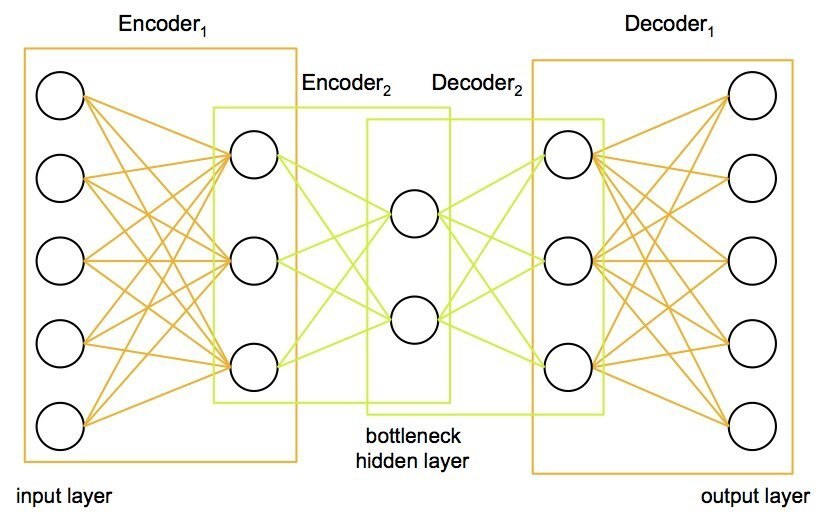
\includegraphics[width=0.7\textwidth]{stacked_ae}
  \end{center}
  \caption{Architettura di un \textit{stacked autoencoder}}
  \label{fig:stacked_ae}
\end{figure}
Gli \textit{autoencoder} come quello in figura~\ref{fig:semplice_ae} hanno dato risultati equiparabili, se non migliori, a quelli ottenuti con metodi di \textit{dimensionality reduction} classici (\textit{cfr}. \cite{ng_sparse_ae},\cite{pca_vs_ae_1}).
Essendo gli AE delle reti neurali, è possibile aggiungere vari strati densi, come si vede in figura~\ref{fig:stacked_ae}.
Questi \textit{autoencoder} prendono il nome di AE multi-strato o \textit{stacked autoencoder} ed hanno capacità astrattive maggiori. % TODO stai attento
Allo stesso modo è anche possibile aggiungere strati convolutivi, convolutivi trasposti oppure di \textit{down} e di \textit{up-sampling}.

\paragraph{Strati Convolutivi}
Un \textit{convolutional layer} è uno strato in cui i pesi hanno la forma di un filtro convolutivo, in questo modo verrà mantenuta anche dell'informazione spaziale.
In pratica la rete si adatta in modo che i filtri lascino passare, o mettano in evidenza, soltanto quelle caratteristiche utili allo svolgimento del compito.
Come viene mostrato molto bene in \cite{conv_arithm}, questo tipo di convoluzioni è una generalizzazione parametrica delle convoluzioni descritte a pagina \pageref{conv_para}.

Innanzitutto è bene elencare i parametri che caratterizzano uno strato di questo tipo, per semplicità si suppone che le immagini ed i \textit{kernel} utilizzati siano sempre quadrati:
\begin{itemize}
  \item $n$ indica il lato dell'immagine in ingresso;

  %\item $m$ indica il lato dell'immagine in uscita;

  \item $k$ indica il lato del filtro.
    Si ricorda che i valori all'interno del filtro sono i pesi che dovranno essere imparati;

  \item $p$ indica quanto \textit{zero padding} aggiungere all'immagine in ingresso.
    Con \textit{zero padding} si intende l'aumentare la dimensione dell'input aggiungendo righe e colonne di zeri.
    Il risultato dell'applicazione del \textit{padding} con $p=1$ può essere osservato in figura~\ref{fig:conv_layer_1ch_p1_s2};

  \item $s$ indica il passo, in inglese \textit{stride}, con cui il filtro viene mosso sull'immagine in ingresso.
    In figura~\ref{fig:conv_layer} sono riportati i risultati che si ottengono con passi differenti;

  \item con $ch_{in}$ si specifica quanti sono i canali in ingresso, ad esempio se l'immagine in \textit{input} è in scala di grigi si avrà $ch_{in} = 1$;

  \item con $ch_{out}$ si specifica quanti sono i canali in uscita.

\end{itemize}
% TODO
%Fissata un valore $k$ per la dimensione del \textit{kernel}, in figura~\ref{fig:conv_layer_1ch} $k=3$, 
L'equazione \ref{eq:conv} mostra la relazione che intercorre tra i vari parametri dello strato convolutivo e la dimensione $m$ dell'immagine in uscita.
\begin{equation} \label{eq:conv}
  m = \frac
  {n + 2p - f}
  {s} 
  + 1
\end{equation}
Si fa notare che le convoluzioni descritte a pagina \pageref{conv_para} equivalgono ad impostare, con $k$ dispari, i parametri $p=\lfloor k/2 \rfloor$, $s=1$, $ch_{in}=1$ (oppure 3 a seconda del caso) e $ch_{out}=1$.
Infatti l'immagine in uscita che si ottiene ad esempio con l'operatore Sobel ha dimensioni pari a quelle dell'immagine in ingresso.

Osservando le architetture delle reti convolutive VGG~\cite{vgg} e ResNet~\cite{resnet} ci si accorge che, fatta eccezione per i primi \textit{layer}, gli strati hanno un numero di canali in ingresso ed in uscita dell'ordine delle centinaia.
Nel caso del primo \textit{layer} dell'architettura VGG11 si ha $ch_{in} = 3$ e $ch_{out} = 64$, mentre per il secondo si ha $ch_{in} = 64$ e $ch_{out} = 128$.
Una delle motivazioni è che avere più canali significa avere più \textit{kernel}, quindi anche più possibilità di apprendimento.
Infatti, prendendo in considerazione un solo strato convolutivo, il numero di kernel è dato da $n_k = ch_{in}*ch_{out}$, mentre il numero di parametri modificabili durante l'allenamento è $n_k * k * k$.
%Infatti, prendendo in considerazione uno strato convolutivo che prende in ingresso un'immagine in scala di grigi
%Con semplici calcoli si può vedere come il numero di parametri 
% TODO nota sul numero di parametri da imparare 
% TODO cosa manca da dire??

% TODO magari si può mettere in modo più carino
\begin{figure}[ht]
  \begin{center}
  \begin{tabular}{cc}
    \begin{subfigure}{.49\linewidth}
      \centering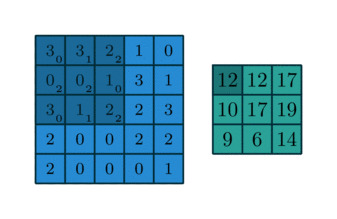
\includegraphics[width=\textwidth]{conv_example}
      \caption{$ch_{out}=1$, $p=0$ e $s=1$}
      \label{fig:conv_layer_1ch}
    \end{subfigure} &

    \begin{subfigure}{.49\linewidth}
      \centering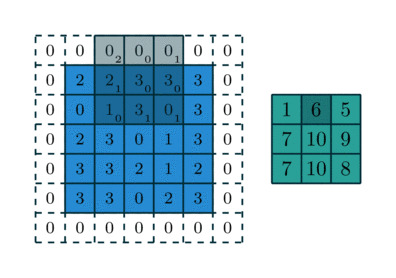
\includegraphics[width=\textwidth]{conv_example_1}
      \caption{$ch_{out}=1$, $p=1$ e $s=2$}
      \label{fig:conv_layer_1ch_p1_s2}
    \end{subfigure}

    %\begin{subfigure}{.45\linewidth} % TODO
    %  \centering\includegraphics[width=\textwidth]{example-image} % mettere immagine con volumi simile a quella di Ng nel video
    %  \caption{A tre canali}
    %  \label{fig:conv_layer_3ch}
    %\end{subfigure}

  \end{tabular}
  \caption{Esempio di strati convolutivi}
  \label{fig:conv_layer}
  \end{center}
\end{figure}

\paragraph{Strati di Down-Sampling}
È stato dimostrato empiricamente che inserire degli strati il cui compito è ridurre le dimensioni dell'\textit{input}, aiuta le reti convolutive ad ottenere risultati migliori.
Infatti sia l'architettura VGG che quella ResNet sfruttano ampiamente un tipo di \textit{layer} chiamato Max-Pooling.
Quest'ultimo, osservabile in figura~\ref{fig:pool_layer}, assomiglia ad un \textit{convolutional layer} ma non ha parametri apprendibili.
Infatti il filtro ritorna semplicemente il massimo dell'area su cui è stato posizionato.
La dimensione del \textit{kernel} e lo \textit{stride} scelto definiscono la dimensione dell'output.
Solitamente uno strato di questo tipo viene utilizzato per dimezzare $n$, cioè è ottenibile impostando $k=2$ e $s=2$.

\begin{figure}
\centering
\begin{minipage}{.65\textwidth}
  \centering
  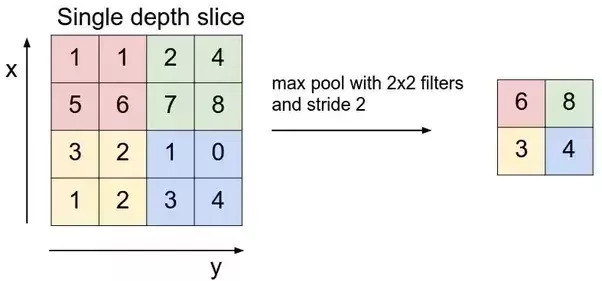
\includegraphics[width=\linewidth]{max-pool}
    \caption{Esempio di strato max-pooling}
    \label{fig:pool_layer}
\end{minipage}%
\begin{minipage}{.35\textwidth}
  \centering
  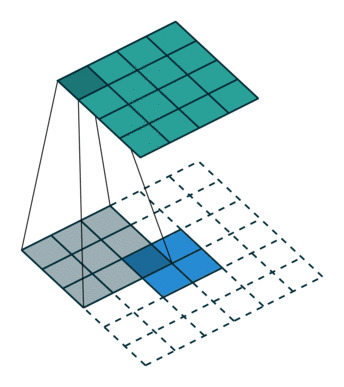
\includegraphics[width=.9\linewidth]{conv-transposed}
    \caption{Esempio di strato convolutivo trasposto}
    \label{fig:conv-transposed}
\end{minipage}
\end{figure}

Fin'ora sono stati descritti gli strati comuni a tutte le reti convolutive, ora verranno illustrati due \textit{layer} elusivi degli \textit{autoencoder}.

\paragraph{Strati di Up-Sampling}
Come il nome suggerisce, lo Up-Sampling \textit{layer} effettua un'operazione opposta a quella di uno strato di Down-Sampling.
Nello specifico aumenta le dimensioni dell'\textit{input} riempendo gli spazi creati con medie tra gli elementi esistenti oppure ripetendoli.

\paragraph{Strati Convolutivi Trasposti}
Lo scopo di questi strati è simulare l'opposto di un'operazione convolutiva: se una convoluzione riduce la dimensione del dato in ingesso, una convoluzione trasposta deve aumentarlo.
Il modo più semplice per ottenere questo effetto è effettuare una convoluzione con un \textit{zero padding} sufficientemente grande, come si vede in figura~\ref{fig:conv-transposed}.
% TODO spiegare perché trasposto
%Viene usato il termine trasposto perché una convoluzione può 
%\todo[inline]{spiegare come i convolutivi possono essere rappresentati da matrici}


